\documentclass[10pt]{article}
\usepackage[utf8]{inputenc}
\usepackage[english]{babel}
\usepackage[left=2cm, right=2cm, top=2cm, bottom=2cm]{geometry}
\usepackage{amsmath, wrapfig, pgfplots}

\pgfplotsset{compat=1.9}

\begin{document}

\title{Cascaded Approximation of Gaussian Blur}
\author{Vabishchevich Nikolay}
\date{May 8, 2015}
\maketitle


\section{Basic definitions}

\begin{wrapfigure}{r}{0pt}
    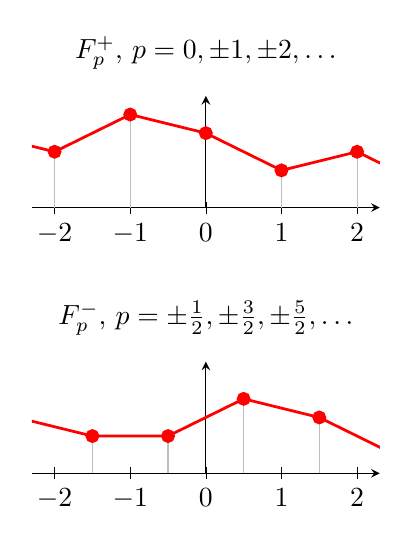
\begin{tikzpicture}
        \begin{axis} [ width = 6cm, height = 3cm, name = plot,
                title = {$F^+_p$, $p = 0, \pm1, \pm2, \ldots$},
                xmin = -2.3, xmax = 2.3, axis x line = bottom,
                xtick = {-2, ..., 2}, x tick style = { color = black },
                ymin = 0, ymax = 6, axis y line = middle, ytick = \empty ]
            \addplot[sharp plot, mark = *, line width = 1pt, red] coordinates
                { (-3, 4) (-2, 3) (-1, 5) (0, 4) (1, 2) (2, 3) (3, 1) };
            \addplot[ycomb, lightgray] coordinates
                { (-2, 3) (-1, 5) (1, 2) (2, 3) };
        \end{axis}
        \begin{axis} [ width = 6cm, height = 3cm,
                at = { (plot.below south) }, anchor = above north, yshift = -0.5cm,
                title = {$F^-_p$, $p = \pm\frac12, \pm\frac32, \pm\frac52, \ldots$},
                xmin = -2.3, xmax = 2.3, axis x line = bottom, xtick = {-2, ..., 2}, x tick style = { color = black },
                ymin = 0, ymax = 6, axis y line = middle, ytick = \empty ]
            \addplot[sharp plot, mark = *, line width = 1pt, red] coordinates
                { (-2.5, 3) (-1.5, 2) (-0.5, 2) (0.5, 4) (1.5, 3) (2.5, 1) };
            \addplot[ycomb, lightgray] coordinates
                { (-1.5, 2) (-0.5, 2) (0.5, 4) (1.5, 3) };
        \end{axis}
    \end{tikzpicture}
\end{wrapfigure}

In this article I'm using two different sets of grid point positions. The first one is grid point at
every integer, $F^+_k$ (I call it even and mark with ``$+$''). The second one is grid points positioned
halfway between adjacent integers, $F^-_{k+1/2}$ (I call it odd and mark with ``$-$'').
Correspondingly there are two types of convolution filters: even
\begin{equation}\label{conv+}
    R^\pm_p = \sum_{k\in Z} F^\pm_{p+k}K^+_k,
\end{equation}
and odd
\begin{equation}\label{conv-}
    R^\mp_p = \sum_{k\in Z} F^\pm_{p+k+\frac12}K^-_{k+\frac12},
\end{equation}
where $K^\pm_p$ is filter kernel. Even filter doesn't change source oddness but odd filter do (hence
the name). Therefore our target problem is to effectively calculate approximation of
\begin{equation}
    R^\pm_p = \sum_{k\in Z} F^\pm_{p+k}G_k,
\end{equation}
where $F^\pm_p$ is the source function and $G_k$ is even gaussian kernel,
\begin{equation}\label{gauss_n}
    G_k = \frac1{\sqrt{2\pi\sigma^2}}\exp\left\{-\frac{k^2}{2\sigma^2}\right\},
\end{equation}
especially for large standard deviation $\sigma$.

The main tool for such task is the Fourier transform. I'm using it in the following form:
\begin{align}
    F^+(\varphi) &= \sum_{k\in Z} F^+_k e^{ik\varphi},\\
    F^-(\varphi) &= \sum_{k\in Z} F^-_{k+\frac12} e^{i(k+\frac12)\varphi},
\end{align}
\begin{equation}
    F^\pm_p = \frac1{2\pi}\int_{-\pi}^\pi F^\pm(\varphi)e^{-ip\varphi}d\varphi.
\end{equation}
As usual, Fourier transform of real function satisfies
\begin{equation}
    F^\pm(-\varphi) = F^{\pm*}(\varphi).
\end{equation}
Also due to discreteness holds the following (another source of the even/odd name):
\begin{equation}
    F^\pm(\varphi+2\pi) = \pm F^\pm(\varphi).
\end{equation}
For symmetric (relative to 0) functions its Fourier amplitude is strictly real.

For convolutional filter with even kernel $K^+_p$ (\ref{conv+}) holds
\begin{equation}
    R^\pm(\varphi) = F^\pm(\varphi)K^{+*}(\varphi).
\end{equation}
In case of odd kernel $K^-_p$ (\ref{conv-}),
\begin{equation}
    R^\mp(\varphi) = F^\pm(\varphi)K^{-*}(\varphi).
\end{equation}
For symmetric filters it's possible to drop conjugation sign in these equations.

In the following I'll need transforms of basic binomial filters. That's well known sequence of
filters, kernels of which from the beginning of the sequence look like
\begin{align}
    B^1 &= [1, 1] / 2,\\
    B^2 &= [1, 2, 1] / 4,\\
    B^3 &= [1, 3, 3, 1] / 8,\\
    B^4 &= [1, 4, 6, 4, 1] / 16,\\
    B^5 &= [1, 5, 10, 10, 5, 1] / 32,\\
    B^6 &= [1, 6, 15, 20, 15, 6, 1] / 64,\\
            &\cdots\nonumber
\end{align}
Filters from the sequence at even index is even and of odd index is odd. Also it's easy to see that
effect from high order filter $B^n$ is the same as from the first filter $B^1$ (or simply $B$) applied
$n$ times. Hence its Fourier transform is
\begin{equation}
    B^n(\varphi) = \cos^n(\varphi/2).
\end{equation}

\begin{wrapfigure}{r}{0pt}
    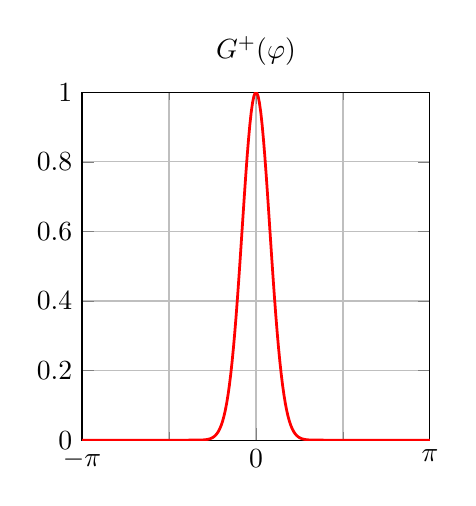
\begin{tikzpicture}
        \begin{axis} [ title = $G^+(\varphi)$, width = 6cm, height = 6cm,
            domain = -1:1, samples = 256,
            xtick = {-1, 0, 1}, xticklabels = {$-\pi$, $0$, $\pi$}, minor x tick num = 1,
            xmin = -1, xmax = 1, xminorgrids = true, xmajorgrids = true,
            ymin = 0, ymax = 1, yminorgrids = true, ymajorgrids = true ]
            \addplot[sharp plot, line width = 1pt, red] {exp(-8*(x*pi)^2)};
        \end{axis}
    \end{tikzpicture}
\end{wrapfigure}

Going back to our gaussian filter (\ref{gauss_n}), its Fourier transform is another gaussian function
\begin{equation}\label{gauss}
    G^+(\varphi) \approx \exp\left\{-\frac{\sigma^2\varphi^2}2\right\}.
\end{equation}
That function has two different regions. The first is almost zero at high frequency and the second
is bell-like shape at low frequency. Correspondingly the task of approximation can be divided into
two subtasks described in the following sections.



\end{document}
